\section{Executed operation and its exact scope}

\subsection{A directed four-state fixture}
The executed fixture has $B=\{2,3\}$ and, with $d=2^{-100}$ and $a=1-3d$,
\[
\pi=(2a/3,\ a/3,\ d,\ 2d).
\]
At physical rate one it resets to $\pi$. Add the directed cycle
$0\to2\to1\to3\to0$, with rate $d/\pi(x)$ at state $x$.
Every cycle edge carries flux $d$, so $\pi$ is invariant while detailed
balance fails. The reset gives symmetrized gap at least one. We use $R=4$,
$g=1/4$, $\zeta=d$, initial state $0$, window $H=5$, and mesh $2^{-10}$
in normalized time.

This is a deliberately small supplied model, not an acquired natural system.
Its static probability and conditional rare-state draw are elementary exact
operations. The general correlated Gibbs static algorithm is not re-executed.
The exact four-state solver is the appropriate baseline and is faster here.
The fixture tests the new dynamic conditional path, directional history,
arbitrary-start branch and huge finite clock.

The diagnostic uses $b=320$ and $L=65536$, with the instance certificate
\eqref{eq:instance}. It makes 4096 Palm calibration proposals, then generates
1024 accepted conditional records and their observed initial segments.
Native kernel choices use integer rational probabilities. Block clock counts,
order statistics and window extraction use standard floating Poisson,
gamma and binomial implementations. This last choice is an explicit execution
limit: their distribution errors are not certified by the general finite-clock
proof. A seeded pseudorandom generator supplies reproducibility rather than
literal independent physical random bits.

\begin{center}
\begin{tabular}{lr}
\toprule
Quantity & Executed or exact value\\
\midrule
Stationary failure probability & $2.3665827156630354\times10^{-30}$\\
Exact mean first-event time from state $0$ & $2.5353012004564588\times10^{29}$\\
Exact $q_G$ & $6.4618554975047656\times10^{-26}$\\
Acquired $\widehat q_G$ & $6.474837356056015\times10^{-26}$\\
Observed relative parameter error & $+0.002008998585$\\
Exact Palm mean & $0.4166285202760781$\\
Acquired Palm mean & $0.4174655263838020$\\
Empirical entry-transition TV & $0.01985677083$\\
Empirical event-time Kolmogorov distance & $0.03047888737$\\
Sample mean / exact mean & $1.04116720427$\\
\bottomrule
\end{tabular}
\end{center}
Times are in model units, not a measured physical lifetime. The empirical TV
entry compares four entry categories; it is not a TV estimate of the entire
path law.

The acquired mean is exactly the rational histogram statistic
$19903051489/47675916288$. The reference probability and lifetime were not
supplied to calibration or to the generated geometric clocks. They were
loaded only for subsequent comparisons.

\subsection{Finite schedule evidence, without overstating the diagnostic}
The rational radius $27/1024$ gives the mean interval
$[0.391098338883802,\ 0.443832713883802]$.
For ideal independent Palm draws, Hoeffding gives a failure bound
$2e^{-729/128}$. Bounding that exponential by a finite positive rational
Taylor sum gives the certified upper bound $0.00676317<0.01$.
This statement is conditional on the ideal clock distribution, as just
distinguished from the floating diagnostic.

A rational mixing certificate is $\eta\le2^{-14}$: $\log 2<7/10$ follows
from the first four terms of the exponential series, and
$gb=80\ge(100+14)(7/10)$. Inserting the observed mean lower bound and exact
$p$ into \eqref{eq:instance} bounds the structural error by
$0.01282038$. The same mean interval bounds geometric-parameter TV by
$0.06741831$. Their sum is $0.08023869$, before finite primitive errors.
It is a legitimate certificate for ideal block draws, not an end-to-end
certification of the standard-library floating samplers.

Using exact reference values only as an independent analytic comparison,
\eqref{eq:struct} is $0.00505584263$. That smaller number is not used to
calibrate $\widehat q_G$.

\subsection{A separately executed finite-bit huge clock}
The actual clock attached to all 1024 records uses the integer implementation
\texttt{finite\_geometric.py}. Its input is the acquired rational
\[
\widehat q_G=
\frac{1304386285434593}
     {20145467966304672880072387975829149188096}.
\]
The per-draw clock tolerance is $2^{-24}$. The compiler stores 89 fixed-point
powers, uses 205 fractional bits and consumes 116 fresh fair bits per draw
in its mathematical model. It never loops over the failed-block index.
The cap is
$370665681317113387681080266$, with an 89-bit index encoding.
Every TV component and their sum are checked by exact rational arithmetic.

The 1024 clock draws used 3,808,709 fixed-point multiplications, 90,446 CDF
queries and 118,784 pseudorandom bits, taking about $0.97$ seconds in this
run. The theorem-level guarantee assumes unbiased independent bits;
the arithmetic and finite-work bounds do not depend on the seed.
Large calendar bin indices are serialized as decimal strings and combined
with the local bins using integer arithmetic, avoiding floating conversion
of the enormous waiting time.

\subsection{The complete executed bill}
The native block run made 428,007,591 forward/reverse updates, including
268,446,811 calibration updates and 327,003 initial-prefix updates.
There were 6526 proposals in total, 998,834,361 native 64-bit pseudorandom
words, 214,033,844 integer categorical calls, 7550 Poisson calls,
13,052 gamma calls and 1024 binomial calls. Integer rejection retries are
recorded separately (35,680,481). The block run took $12.31$ seconds on
this executor, of which $7.63$ seconds was calibration. No observed initial
segment failed. The explicit proposal, event-count and integer-rejection caps, and all
output paths, are retained with the code. Internal rejection loops in the
standard-library floating distributions are not a certified worst-case
finite primitive; the theorem uses the separate rational compiler.

The independently constructed exact reference used 180-digit arithmetic
and a two-by-two killed matrix. It completed in about $0.09$ seconds.
The general theorem's conservative uniform recipe at
$\eps=0.1,\delta=0.01$ instead prescribes $b=444$, $L=18,472,960$,
67,108,864,000 calibration proposals and about
$1.2397\times10^{18}$ leading local updates. That uniform schedule was
\emph{not} executed. Its cost is sufficient, not necessary; the instance
certificate supplies the smaller diagnostic schedule without claiming an
economical general implementation.

\subsection{Algebra and direction checks}
An independent exact-rational enumeration verified the Palm density on all
1364 state paths with zero through four potential updates in a nontrivial
four-state instance. Every residual is exactly zero. Substituting the forward
kernel for its reversal gives a conditional-path TV discrepancy about $0.45$
in these finite enumerations.

For the rare fixture, the correct first-entry transition probabilities
approach $(1/3,1/15,4/15,1/3)$ for the ordered categories
$(0\to2,1\to2,0\to3,1\to3)$. The incorrect stationary boundary
reconstruction based on outgoing rather than incoming dynamics differs
from the exact first-entry law by TV $0.4$ up to the displayed
$10^{-30}$-scale corrections. This is a reference calculation, not a second
large run of the wrong algorithm.

\begin{figure}[htbp]
\centering
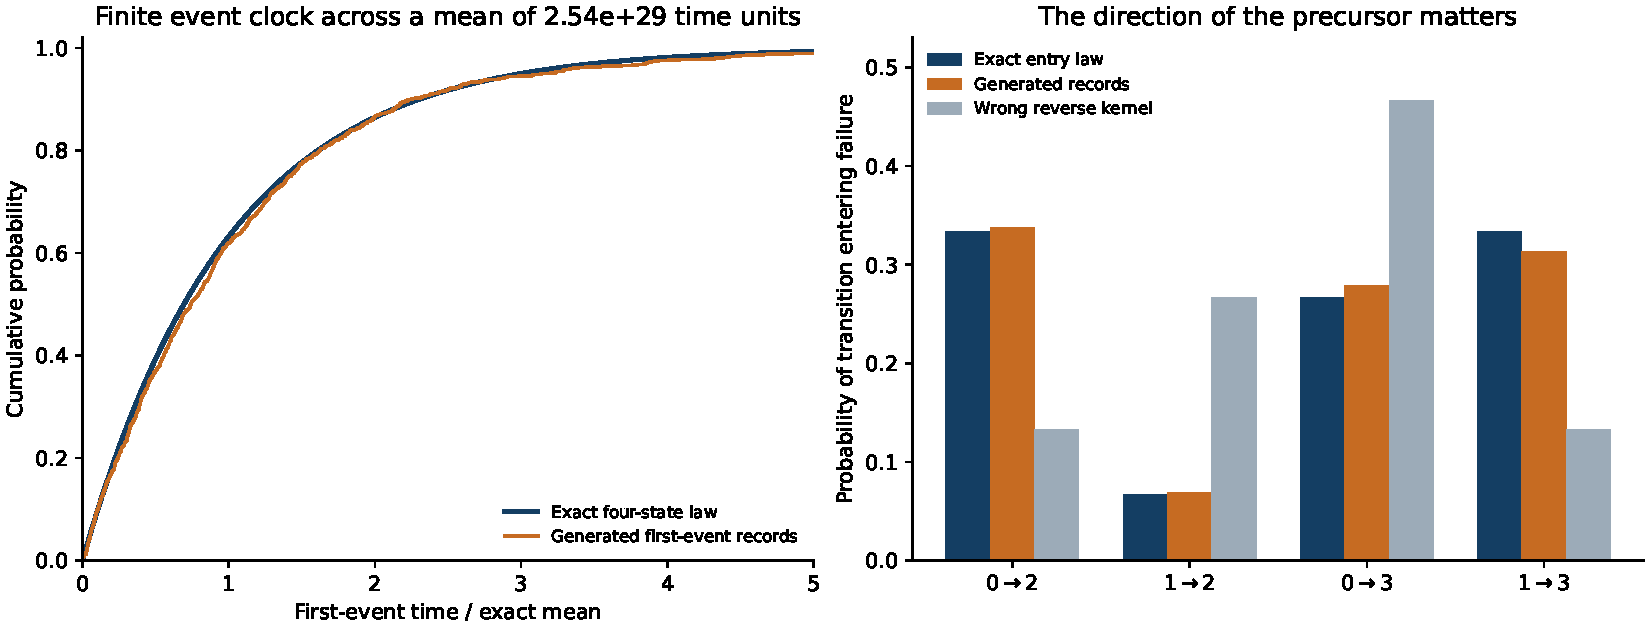
\includegraphics[width=\linewidth]{../next4_execution/event_law_diagnostic.pdf}
\caption{Executed supplied-model diagnostic. Left: generated finite-clock
first-event records against the independent exact law. Right: the entry
transition distribution, including the incorrect boundary reconstruction
that uses the wrong time direction. The small exact solver is a stronger
baseline for this fixture; the plot does not establish practical advantage
for a general exponentially large state space.}
\end{figure}
